% L13a jump hidden Markov model, one simulated day: the N states ordered from the most
% negative to the most positive daily growth rate, each with its Student-t emission. An
% ordinary day steps with the counted transition matrix. On a day with no episode under
% way, a jump episode starts with probability epsilon and lasts a Poisson number of days
% with mean lambda; each episode day draws its state from the most negative states (with
% probability p_neg) or from the most positive states.
%
% Layout ported from the INFORMS 2026 talk (varnerlab/INFORMS-Annual-Meeting-2026-Varnerlab,
% talk/figs/jumphmm_architecture.tex, also Fig. jumphmm of the paper). November 12, 2026:
% redrawn in the style of the week-12 schematics (jumphmm-diagram.tex), and the two arc
% labels now use p_neg, the symbol of the lecture's sampling algorithm.
\documentclass[tikz,border=6pt]{standalone}
% Shared style for the L13a schematics (November 12, 2026), \input by each Fig-L13a-*.tex.
% Same fonts, ink, accent colors, boxes, and arrows as the L12a schematics
% (week-12/L12a/figs/abm-diagram.tex), with the plot styles of the L10b profit diagrams
% (arrowed axes, a thick ink curve, open circle markers, dashed drops). The notebook SVG
% carries a dark palette added by theme_svg.py; every color here must be mapped there.
\usepackage[no-math]{fontspec}
\IfFontExistsTF{Arial}{\setsansfont{Arial}}{\setsansfont{TeX Gyre Heros}}
\renewcommand{\familydefault}{\sfdefault}
\usepackage{amsmath,amssymb}
\usetikzlibrary{arrows.meta,calc,positioning,decorations.pathreplacing}

\definecolor{vnink}{HTML}{202124}
\definecolor{gdblue}{HTML}{0091FF}
\definecolor{gdred}{HTML}{E02020}
\definecolor{gdgray}{HTML}{6D7278}
\definecolor{saorange}{HTML}{F08C00}
\definecolor{boxfill}{HTML}{F1F3F4}
\definecolor{orangefill}{HTML}{FFE8C7}
\definecolor{bluefill}{HTML}{E5F3FF}
\definecolor{redfill}{HTML}{FDE8E8}
\definecolor{gridgray}{HTML}{E3E5E8}

\tikzset{
  every picture/.append style={x=1cm, y=1cm, font=\sffamily\small, text=vnink},
  % boxes and arrows, as in the L12a schematics
  flow/.style={draw=vnink, line width=0.9pt, -{Latex[length=2.4mm, width=1.7mm]}},
  feedback/.style={draw=saorange, line width=1.2pt, -{Latex[length=2.6mm, width=1.9mm]}, rounded corners=6pt},
  sumbox/.style={draw=vnink, fill=boxfill, line width=0.8pt, rounded corners=3pt, inner sep=5pt, align=center},
  note/.style={text=gdgray, font=\sffamily\footnotesize, align=center},
  state/.style={circle, draw=vnink, fill=white, line width=1.0pt, minimum size=1.1cm, inner sep=0pt, font=\sffamily\normalsize},
  % plots, as in the L10b profit diagrams
  axis/.style={draw=vnink, line width=0.8pt, -{Latex[length=2.6mm, width=1.8mm]}},
  spine/.style={draw=vnink, line width=0.8pt},
  curve/.style={draw=vnink, line width=1.6pt, line join=round, line cap=round},
  series/.style={draw=gdgray, line width=0.9pt, line join=round},
  drop/.style={draw=gdgray, line width=0.8pt, dash pattern=on 3pt off 2pt},
  pt/.style={circle, draw=vnink, fill=white, line width=1.0pt, inner sep=0pt, minimum size=2.0mm},
}


\begin{document}
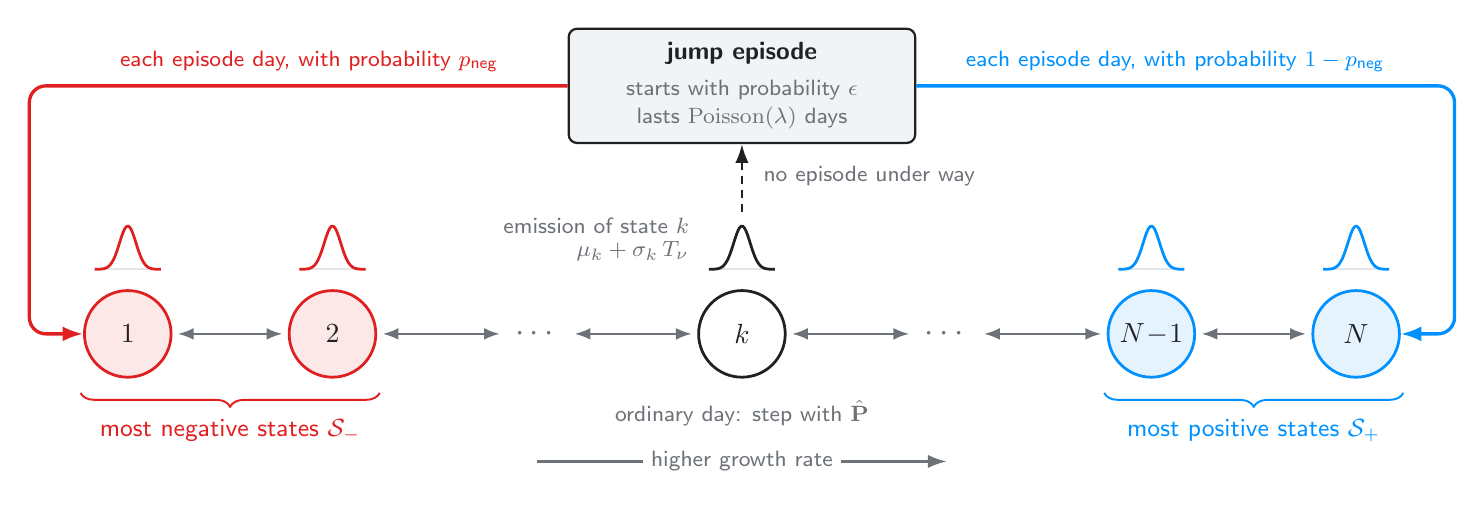
\begin{tikzpicture}[
  markov/.style={draw=gdgray, line width=0.8pt, {Latex[length=2.0mm, width=1.5mm]}-{Latex[length=2.0mm, width=1.5mm]},
                 shorten <=2pt, shorten >=2pt},
  jump/.style={line width=1.2pt, -{Latex[length=2.6mm, width=1.9mm]}, rounded corners=6pt},
]
  % the chain: the most negative states, state k, and the most positive states
  \node[state, draw=gdred, fill=redfill]   (s1)   at ( 0.0, 0) {$1$};
  \node[state, draw=gdred, fill=redfill]   (s2)   at ( 2.6, 0) {$2$};
  \node[text=gdgray, font=\sffamily\large] (ld)   at ( 5.2, 0) {$\cdots$};
  \node[state]                             (sk)   at ( 7.8, 0) {$k$};
  \node[text=gdgray, font=\sffamily\large] (rd)   at (10.4, 0) {$\cdots$};
  \node[state, draw=gdblue, fill=bluefill] (sNm1) at (13.0, 0) {$N\!-\!1$};
  \node[state, draw=gdblue, fill=bluefill] (sN)   at (15.6, 0) {$N$};
  \draw[markov] (s1) -- (s2);
  \draw[markov] (s2) -- (ld);
  \draw[markov] (ld) -- (sk);
  \draw[markov] (sk) -- (rd);
  \draw[markov] (rd) -- (sNm1);
  \draw[markov] (sNm1) -- (sN);

  % the emission of each state: a bell above it
  \foreach \x/\c in {0.0/gdred, 2.6/gdred, 7.8/vnink, 13.0/gdblue, 15.6/gdblue} {
    \draw[draw=gridgray, line width=0.6pt] ({\x - 0.42}, 0.82) -- ({\x + 0.42}, 0.82);
    \draw[draw=\c, line width=1.0pt]
      plot[domain=-0.42:0.42, samples=40, smooth, variable=\t] ({\x + \t}, {0.82 + 0.55*exp(-\t*\t/0.022)});
  }
  \node[note, anchor=east, align=right] at (7.25, 1.2) {emission of state $k$\\[-1pt]$\mu_{k}+\sigma_{k}\,T_{\nu}$};
  \node[note, anchor=north] at (7.8, -0.72) {ordinary day: step with $\hat{\mathbf{P}}$};

  % a jump episode starts on a day with no episode under way
  \node[sumbox, minimum width=4.4cm] (clock) at (7.8, 3.15)
    {\textbf{jump episode}\\[2pt]{\footnotesize\color{gdgray}starts with probability $\epsilon$}\\[-1pt]{\footnotesize\color{gdgray}lasts $\mathrm{Poisson}(\lambda)$ days}};
  \draw[flow, dash pattern=on 3pt off 2pt] (7.8, 1.55) -- (clock.south);
  \node[note, anchor=west] at (7.95, 2.0) {no episode under way};

  % each episode day draws its state from one of the two tails
  \draw[jump, draw=gdred]  (clock.west) -- (-1.25, 3.15) -- (-1.25, 0) -- (s1.west);
  \draw[jump, draw=gdblue] (clock.east) -- (16.85, 3.15) -- (16.85, 0) -- (sN.east);
  \node[anchor=south, text=gdred,  font=\sffamily\footnotesize] at (2.3, 3.2)  {each episode day, with probability $p_{\text{neg}}$};
  \node[anchor=south, text=gdblue, font=\sffamily\footnotesize] at (13.3, 3.2) {each episode day, with probability $1-p_{\text{neg}}$};

  % the two tails and the order of the states
  \draw[decorate, decoration={brace, amplitude=5pt, mirror}, draw=gdred, line width=0.7pt]
    (-0.6, -0.75) -- (3.2, -0.75) node[midway, below=6pt, text=gdred] {most negative states $\mathcal{S}_{-}$};
  \draw[decorate, decoration={brace, amplitude=5pt, mirror}, draw=gdblue, line width=0.7pt]
    (12.4, -0.75) -- (16.2, -0.75) node[midway, below=6pt, text=gdblue] {most positive states $\mathcal{S}_{+}$};
  \draw[draw=gdgray, line width=0.8pt, -{Latex[length=2.4mm, width=1.7mm]}] (5.2, -1.62) -- (10.4, -1.62);
  \node[note, fill=white, inner sep=3pt] at (7.8, -1.62) {higher growth rate};

\end{tikzpicture}
\end{document}
